\documentclass[11pt]{article}
\usepackage[T1]{fontenc}
\usepackage{lmodern}
\usepackage[margin=1in]{geometry}
\usepackage{amsmath,amssymb,amsthm,mathtools}
\usepackage{microtype}
\usepackage{xcolor}
\usepackage{booktabs,enumitem}
\usepackage{needspace,etoolbox}
\usepackage{tikz}
\usetikzlibrary{arrows.meta,positioning,calc}
\usepackage[numbers,sort&compress]{natbib}
\usepackage[colorlinks=true,linkcolor=blue!45!black,citecolor=blue!45!black,urlcolor=blue!45!black]{hyperref}
\usepackage[capitalise,noabbrev]{cleveref}
\newtheorem{theorem}{Theorem}[section]
\newtheorem{lemma}[theorem]{Lemma}
\newtheorem{proposition}[theorem]{Proposition}
\newtheorem{corollary}[theorem]{Corollary}
\theoremstyle{definition}
\newtheorem{definition}[theorem]{Definition}
\theoremstyle{remark}
\newtheorem{remark}[theorem]{Remark}
\BeforeBeginEnvironment{theorem}{\Needspace{6\baselineskip}}
\BeforeBeginEnvironment{lemma}{\Needspace{6\baselineskip}}
\BeforeBeginEnvironment{proposition}{\Needspace{6\baselineskip}}
\BeforeBeginEnvironment{corollary}{\Needspace{6\baselineskip}}
\BeforeBeginEnvironment{remark}{\Needspace{6\baselineskip}}
\renewcommand{\bibsection}{\section*{References}\addcontentsline{toc}{section}{References}}
\newcommand{\Q}{\mathbb Q}
\newcommand{\C}{\mathbb C}
\DeclareMathOperator{\Mat}{Mat}
\DeclareMathOperator{\rank}{rank}
\DeclareMathOperator{\ord}{ord}
\DeclareMathOperator{\Span}{span}
\setlist{itemsep=3pt,topsep=5pt}
\setlength{\emergencystretch}{2em}
\numberwithin{equation}{section}
\title{Polynomial Hitting Lists for Noncommutative Rational Formulas}
\author{OpenAI}
\date{September 24, 2026}
\hypersetup{pdftitle={Polynomial Hitting Lists for Noncommutative Rational Formulas},pdfauthor={OpenAI},pdfsubject={A uniform construction over the rational numbers}}
\begin{document}
\maketitle
\begin{abstract}
We construct, in deterministic polynomial bit time, a polynomial-size list of rational matrix tuples for noncommutative rational formulas over $\Q$ of bounded tree size. Every nonzero admissible formula has a defined, invertible value at one tuple, with no separate bounds on inverse nesting or rational constant heights. Matrix dimensions, entry bit lengths, and total output length are polynomially bounded.
\end{abstract}
\section{Introduction}
\label{sec:introduction}

A noncommutative rational formula is a rooted tree whose leaves are variables or rational constants, whose binary gates are addition or ordered multiplication, and whose unary gates are inversion. Its size is its number of vertices, including leaves and inverse gates. At a tuple of square rational matrices, a scalar is interpreted as a scalar multiple of the identity. Evaluation is defined only when every inverse gate encounters an invertible matrix.

Call a formula \emph{admissible} if it has a defined rational matrix evaluation of some positive dimension, and \emph{nonzero} if one of its defined rational matrix evaluations is nonzero. These operational definitions suffice for the hitting-list theorem; its proof does not need a construction of the free skew field. In particular, algebraic cancellations do not enlarge a formula's domain of evaluation.

Identity testing asks whether an admissible formula is zero at every
defined evaluation. Scalar substitutions cannot answer this question:
for example, $x_1x_2-x_2x_1$ vanishes on all scalar tuples but is
nonzero on matrices. A matrix hitting list is a fixed finite list of
tuples that supplies a defined nonzero evaluation for each nonzero
formula in the prescribed class. Such a list permits testing through
evaluations without access to the formula tree. With inverse gates,
the same tuple must satisfy every domain condition imposed by that
tree, including conditions in branches that later cancel.
In oracle terminology, an undefined evaluation is reported as such;
only defined outputs are tested for zero.

\begin{theorem}\label{thm:main}
There are a deterministic Turing machine $G$ and fixed positive integers $C,k$ with the following property. Given $1^n,1^s$, where $n,s\geq1$, the machine outputs a finite list $\mathcal H_{n,s}$ of $n$-tuples of rational square matrices, in at most $C(n+s+1)^k$ bit operations. The entire output, with signed binary numerators and positive binary denominators, has at most $C(n+s+1)^k$ bits. For every nonzero admissible rational formula $\Phi$ in $n$ variables of size at most $s$, some tuple in $\mathcal H_{n,s}$ is a defined evaluation of $\Phi$ with invertible value.

The same list works for all such formulas, regardless of the bit lengths of their rational constants or their inverse depth. The generator receives no formula, oracle, randomness, or advice.
\end{theorem}

The invertible-value conclusion is stronger than the nonzero-value requirement. All tuples produced below even have one common dimension depending only on $n,s$.

\subsection{Context}
The algebraic setting comes from the theory of rational identities
and universal fields of fractions~\citep{Amitsur66,Cohn06}.
Affine-matrix representations of free-field elements appear in
Cohn and Reutenauer~\citep[Section~3.1]{CR94};
Kaliuzhnyi-Verbovetskyi and Vinnikov give a systematic account of
matrix evaluation domains and rational functions~\citep[Section~2]{KVV10}.
The distinction between a rational function and an expression
representing it matters here: equivalent expressions can impose
different conditions on their intermediate inverses. Our operational
formulation retains the original expression throughout.

For division-free computation, Nisan's coefficient-matrix
characterization made rank a central tool in noncommutative
branching-program complexity~\citep{Nisan91}.
Raz and Shpilka gave deterministic polynomial-time identity testing
with access to a formula or branching program~\citep{RS05}.
Bogdanov and Wee developed randomized black-box matrix evaluation
for bounded-degree noncommutative polynomials~\citep{BW05}, and
Forbes and Shpilka constructed deterministic quasipolynomial-size
matrix hitting sets for noncommutative algebraic branching programs,
a model including division-free formulas~\citep{FS13}.

For computation with division, Hrube\v{s} and Wigderson developed
the rational-formula model and its reduction to linear-matrix
singularity testing~\citep{HW15}. Their inverse-matrix realizations
and tests for the domains of gate subformulas are direct predecessors
of our certificate construction. Deterministic polynomial-time
algorithms with access to the input formula followed from operator
scaling and constructive noncommutative-rank
computation~\citep{GGOW16,GGOW20,IQS18}. These algorithms use the
given coefficients, with their encoding lengths included in the
bit model. Derksen and Makam established polynomial bounds on the
dimensions needed for an admissible rational formula to have a
defined evaluation, and derived randomized polynomial-time rational
identity testing~\citep[Section~6]{DM17}. Small witnesses and
algorithms that depend on the input coefficients leave open the
construction of a universal deterministic list from size bounds alone.

Arvind, Chatterjee, and Mukhopadhyay obtained deterministic
quasipolynomial-size hitting sets for rational formulas of inversion
height two~\citep[Theorem~1.1]{ACM22}.
Their subsequent general result handles unrestricted inverse
nesting with quasipolynomial-size rational matrix hitting
sets~\citep{ACM26}; the quantitative bounds used in this comparison
are Theorem~2, Corollary~3, and the paragraph following Remark~52
of the specified preprint version~\citep{ACM25}. Thus rational matrix outputs and arbitrary
inverse nesting already occur in the preceding literature.
Invertible evaluations are also used in the division-algebra methods
of these works~\citep{ACM22,ACM25}. Their general treatment states a
depth reduction that preserves the input formula's evaluation
domain~\citep[Fact~1]{ACM25}. Theorem~\ref{thm:main} gives polynomial
bounds on construction time, total binary output length, and matrix
dimension.
Its complexity bound concerns generation of the list; the cost of
evaluating an unknown formula with arbitrarily large rational
constants is not included.

The result resolves, over $\Q$, the explicit polynomial-size hitting-set
problem for this formula model, and gives the polynomial matrix
dimension asked for in the conclusion of~\citet{ACM25}.
The proof of Theorem~\ref{thm:main} below establishes all the algebraic and algorithmic
ingredients it uses.

The proof also draws on established methods. The multiplicity
argument for explicit subspace designs of Guruswami and
Kopparty~\citep{GK16}, and the connection between subspace designs,
rank condensers, and dimension expansion studied by Forbes and
Guruswami~\citep{FG15}, provide context for our
construction. The underlying Wronskian calculation is
classical~\citep{BD10}. The common-subspace obstruction to
invertibility belongs to noncommutative-rank
theory~\citep{FR04}, while cyclic division algebras and rank
divisibility underlie the regularity methods of Ivanyos, Qiao,
and Subrahmanyam~\citep{IQS17,IQS18}. We prove the precise expansion,
deformation, and domain statements needed here, without importing
the stronger general algorithms from those works.

\subsection{The construction and its logic}

Write $\Mat_q(F)$ for the $q$ by $q$ matrices over a field $F$.
The bridge from formula evaluation to linear algebra is an
\emph{affine linear pencil}, a matrix
\[
 L(x)=A_0+\sum_{i=1}^n A_ix_i,\qquad A_i\in\Mat_q(\Q),
\]
of order $q$. Its evaluation at matrices $X_i\in\Mat_e(E)$ over an
extension field $E/\Q$ is $A_0\otimes I_e+\sum_iA_i\otimes X_i$.
Call the pencil \emph{feasible} if one such evaluation is invertible.
Tensor products and ranks are taken over the indicated field.

A size-$s$ formula gives at most $s+1$ pencils of order at most
$B=2s+1$. Their simultaneous invertibility certifies that every
inverse occurrence in the original tree is defined and that the
final value is invertible. A nonzero admissible formula has a
matrix evaluation over an extension field satisfying all these
conditions. Section~\ref{sec:encoding} proves this reduction, including
the exact conditions at the inverse gates. The construction therefore
seeks a universal rational list on which each such finite family of
feasible pencils is simultaneously invertible.

Two obstacles remain: obtaining full rank at matrices independent of
the pencil coefficients, and keeping all conditions valid when the
parameters become rational numbers. The proof handles them in the
following order.
\begin{enumerate}
\item Section~\ref{sec:expansion} constructs $n+1$ rectangular
matrices over $\Q[t]$. They act on coefficient vectors of polynomials,
reversing the Taylor expansion about the distinct points $0,\ldots,n$
and weighting the Taylor coefficients by powers of $t$.
A Wronskian bound shows that, for every nonzero subspace of dimension
at most $B$, the sum of its images has dimension greater than $n$
times its dimension, even when the subspace has Laurent-series
coefficients. The resulting test for a feasible
pencil is injective. Padding the test matrices to a common square
order $M$ gives matrices $R_i(t)$ for which every feasible pencil of
order $1\leq q\leq B$ satisfies
\[
 \rank\Bigl(\sum_{i=0}^n A_i\otimes R_i(t)\Bigr)>(q-1)M.
\]
\item Section~\ref{sec:division} uses two further parameters $p,r$
to lift these matrices into a division algebra represented by
$M\times M$ matrices. Ranks of block matrices over this algebra are
multiples of $M$, so the strict inequality forces full rank.
Dividing on the left by the lifted $R_0$ restores the constant term
of an affine pencil. A separate application of the lift turns any
defined nonzero formula evaluation into a defined invertible one
over an extension field. This supplies the feasibility assertion
needed for the certificates in Section~\ref{sec:encoding}.
\item Section~\ref{sec:generator} represents multiplication in a
finite-dimensional rational algebra by rational matrices, thereby
replacing the root of unity used in the lift. All root components
must be invertible simultaneously. For any fixed formula, the
product of their determinant conditions is a nonzero polynomial
of bounded degree in $t,p,r$. A fixed three-dimensional integer
grid detects it. Exact rational arithmetic bounds both the
generation time and the total binary output length.
\end{enumerate}

The witnesses, subspaces, and formula-specific determinant products in this proof certify the construction. None is computed by $G$. In particular, the dimension of an initial witness for a formula has no effect on the generator's resource bounds.

The construction also hits every feasible rational affine pencil
of bounded order; see Corollary~\ref{cor:pencil-hitting}.
In particular, it answers the rational-coefficient version of the
black-box \textsc{Singular} construction question for homogeneous
pencils posed by Garg, Gurvits, Oliveira, and
Wigderson~\citep[Section~6, p.~280]{GGOW20}.
Section~\ref{sec:rank} then treats rectangular affine pencils.
Their \emph{noncommutative rank} is their rank over the free skew
field. Corollary~\ref{cor:rank-detecting-list} constructs a universal
nonadaptive list whose normalized evaluation ranks recover this rank
for every rectangular rational affine pencil with prescribed row,
column, and variable counts. It permits exact matrix-value or
ordinary-rank responses and accounts for their processing costs.

\section{Rectangular tests from subspace expansion}
\label{sec:expansion}

Fix the variable and formula-size bounds $n,s\geq1$. We construct
rectangular matrices $T_0,\ldots,T_n$ such that
$\sum_{i=0}^n A_i\otimes T_i$ is injective whenever
$A_0+\sum_{i=1}^n A_i x_i$ is a feasible affine pencil of order
at most $2s+1$. The construction uses an indeterminate $t$; no
specialization of a formal Laurent series will be needed. Set
\begin{equation}\label{eq:parameters}
\begin{gathered}
w=n+1,\qquad B=2s+1,\qquad \Delta=2w^3B,\\
M=\min\{2^a:a\in\mathbb Z_{\geq0},\ 2^a>B\Delta\},
\qquad N=M-\Delta.
\end{gathered}
\end{equation}
The bound $B$ will accommodate all certificate pencils in
Proposition~\ref{prop:formula-certificates}. The padding width $\Delta$
provides the expansion margin, while $M>B\Delta$ makes the eventual
rank deficit smaller than one block. These choices give
$1\leq N<M\leq2B\Delta$.

For a field $K$ and an integer $d\geq 1$, let
\[
  \mathcal P_d(K)=\{f\in K[z]:\deg f<d\},
\]
with its monomial basis.  Put $F=\Q((t))$ and $\mathcal O=\Q[[t]]$.
For $0\leq i\leq n$, define an $F$-linear map
$T_i\colon\mathcal P_N(F)\longrightarrow\mathcal P_M(F)$ by
\begin{equation}
  f=\sum_{a=0}^{N-1}c_{ia}(f)(z-i)^a,
  \qquad
  T_i f=\sum_{a=0}^{N-1}c_{ia}(f)t^a(z-i)^{M-1-a}.
  \label{eq:rectangular-test}
\end{equation}
The exponents in the output are nonnegative and distinct.  Since each
$t^a$ is nonzero in $F$, every $T_i$ is injective.  Its matrix in the
monomial bases has entries in $\mathbb Z[t]$.  More explicitly, its column
corresponding to $z^b$, for $0\leq b<N$, is the coefficient vector of
\begin{equation}
  T_i(z^b)=\sum_{a=0}^{b}\binom{b}{a}i^{b-a}t^a(z-i)^{M-1-a}.
  \label{eq:test-column}
\end{equation}
Thus all its entries have $t$-degree at most $N-1$.  Let $R_i(t)$ be the
$M\times M$ matrix obtained by appending $M-N$ zero columns to $T_i$.

The conclusion of this section is the following proposition.

\begin{proposition}[Rectangular rank bound]
\label{prop:rectangular}
Let $1\leq q\leq B$ and $A_0,\ldots,A_n\in\Mat_q(\Q)$.  Suppose that,
for some extension field $E/\Q$, some integer $e\geq1$, and some
$X_1,\ldots,X_n\in\Mat_e(E)$, the matrix
\[
  A_0\otimes I_e+\sum_{i=1}^n A_i\otimes X_i
\]
is invertible.  Then $\sum_{i=0}^n A_i\otimes T_i$ is injective over $F$,
and
\begin{equation}
  \rank_{\Q(t)}\left(\sum_{i=0}^n A_i\otimes R_i(t)\right)
  \geq qN>(q-1)M.
  \label{eq:padded-rank}
\end{equation}
\end{proposition}

We prove the proposition by showing that the maps $T_i$ jointly expand
every nonzero subspace of dimension at most $B$.  Two elementary facts will
control the vanishing orders of their leading coefficients.
The ordinary-Wronskian multiplicity method used in the subspace designs
of Guruswami and Kopparty~\citep[Section~5.1 of the preprint]{GK16}
is a predecessor of this argument. Their construction bounds
intersections with multiplicity subspaces; here Taylor reversal
relates the vanishing sequences of the input and image spaces.
Forbes and Guruswami~\citep{FG15} explain broader connections among
subspace designs, rank condensers, and dimension expansion.
The lossless and unbalanced dimension expanders of Guruswami, Resch,
and Xing~\citep{GRX18} provided a comparison for the required
small-subspace expansion parameters during development.  Their
linearized-polynomial construction is not used here.
We prove the order estimate and the rectangular expansion statement
directly for the maps above.

\subsection{Vanishing orders and integral reduction}

Let $V\subseteq\mathcal P_d(\Q)$ have dimension $h\geq1$.  Row reduction
of Taylor coefficient vectors about $z=i$ gives a basis with distinct
vanishing orders
\[
  0\leq d_{i1}<\cdots<d_{ih}<d.
\]
These orders describe the entire vanishing filtration: for every integer
$r\geq0$,
\begin{equation}
  \dim_{\Q}\{f\in V:(z-i)^r\text{ divides }f\}
  =\#\{j:d_{ij}\geq r\}.
  \label{eq:vanishing-filtration}
\end{equation}
Indeed, in a nonzero linear combination of the echelon basis, the first
basis vector with a nonzero coefficient supplies its lowest Taylor term.

The leading-term Wronskian computation in the following lemma is
classical; the echelon-basis and Vandermonde argument is also presented
by Bostan and Dumas~\citep[Lemmas~1--3]{BD10}.

\begin{lemma}[Wronskian order bound]
\label{lem:wronskian-orders}
With the notation above, at the $w=n+1$ points $0,\ldots,n$ one has
\begin{equation}
  \sum_{i=0}^n\sum_{j=1}^h d_{ij}
  \leq h(d-1)+w\binom{h}{2}.
  \label{eq:wronskian-bound}
\end{equation}
\end{lemma}

\begin{proof}
For a basis $f_1,\ldots,f_h$ of $V$, consider its Wronskian
\[
  \mathcal W(z)=\det\bigl(f_j^{(r)}(z)\bigr)_{
       0\leq r<h,\,1\leq j\leq h}.
\]
Changing the basis multiplies $\mathcal W$ by a nonzero rational
constant.  At a fixed point $i$, use the echelon basis and write
$f_j=\alpha_j(z-i)^{d_{ij}}+$ higher powers, where $\alpha_j\neq0$.
The contribution of these leading terms to the determinant is
\[
  \left(\prod_{j=1}^h\alpha_j\right)
  \det\bigl((d_{ij})_r\bigr)_{
       0\leq r<h,\,1\leq j\leq h}
  (z-i)^{\sum_jd_{ij}-\binom h2},
\]
where $(X)_r=X(X-1)\cdots(X-r+1)$ and $(X)_0=1$.  Because these are
monic polynomials of successive degrees, the displayed coefficient
determinant is the Vandermonde
$\prod_{a<b}(d_{ib}-d_{ia})$, which is nonzero.  Terms using a higher
power from any $f_j$ have strictly larger total exponent, or vanish on
differentiation.  The displayed exponent is nonnegative because the
$d_{ij}$ are distinct nonnegative integers.  Consequently
\[
  \ord_{z=i}\mathcal W
  =\sum_{j=1}^h d_{ij}-\binom h2,
\]
and in particular $\mathcal W$ is not the zero polynomial.

Each entry in its determinant has degree at most $d-1$, so
$\deg\mathcal W\leq h(d-1)$.  The sum of its vanishing orders at the
distinct points $0,\ldots,n$ is at most its degree.  This gives
\eqref{eq:wronskian-bound}.
\end{proof}

For a subspace $U\subseteq F^D$, define its reduction by
\[
  \overline U
  =\{u\bmod t:u\in U\cap\mathcal O^D\}\subseteq\Q^D.
\]
It is important here to use all integral vectors of the subspace, not
merely the reductions of an arbitrarily chosen basis.

\begin{lemma}[Integral bases of Laurent-series subspaces]
\label{lem:integral-reduction}
Every $k$-dimensional subspace $U\subseteq F^D$ has a basis
$u_1,\ldots,u_k\in\mathcal O^D$ whose reductions are linearly independent.
For such a basis,
\begin{equation}
  U\cap\mathcal O^D=\bigoplus_{j=1}^k\mathcal O u_j,
  \qquad
  \dim_{\Q}\overline U=k.
  \label{eq:integral-lattice}
\end{equation}
\end{lemma}

\begin{proof}
We first construct the basis by induction on $k$, the case $k=0$ being
immediate.  Multiply a nonzero vector of $U$ by a power of $t$ so that
all its coordinates are integral and some coordinate is a unit.  Call
this vector $u_1$ and its unit coordinate $c$.  The subspace of $U$
whose $c$-th coordinate is zero has dimension $k-1$.  By induction it
has an integral basis with independent reductions.  All those
reductions have zero $c$-th coordinate, whereas the reduction of $u_1$
does not.  Together they are therefore independent and form a basis
of $U$ over $F$.

Some $k\times k$ coordinate minor of the resulting basis matrix is a
unit in $\mathcal O$.  If an $F$-linear combination of its columns is
integral, restriction to those coordinates and inversion of that minor
show that all its coefficients belong to $\mathcal O$.  This proves
the first assertion of \eqref{eq:integral-lattice}; reducing its
coefficients modulo $t$ proves the second.
\end{proof}

For a nonzero vector $f$ with Laurent-series coordinates, let
$\nu_t(f)$ denote the minimum of their $t$-valuations.  Its
\emph{leading reduction} is the nonzero vector
$t^{-\nu_t(f)}f\bmod t$.  Any invertible coordinate change over $\Q$
preserves both the integral lattice and this minimum valuation: the
change-of-basis matrix and its inverse both have entries in $\mathcal O$.
In particular, this applies to conversion between monomial and Taylor
coordinates.  All these statements concern formal series and require
no convergence assumption.

\subsection{Expansion of every small subspace}

For an integral input having a unit Taylor coefficient with index $a\leq A$,
the leading reduction of its image uses only indices $a\leq A$; reversal
turns these into output orders at least $M-1-A$. The Wronskian bound then
rules out too small a common image space. The proof below applies this
observation to a suitable subspace for each vanishing order.

\begin{lemma}[Small-subspace expansion]
\label{lem:small-expansion}
For every $k$-dimensional subspace $U\subseteq\mathcal P_N(F)$ with
$1\leq k\leq B$,
\begin{equation}
  \dim_F\left(\sum_{i=0}^n T_iU\right)>(w-1)k.
  \label{eq:small-expansion}
\end{equation}
\end{lemma}

\begin{proof}
Put $W=\sum_{i=0}^nT_iU$ and $\ell=\dim_FW$.  Since $T_0$ is
injective, $\ell\geq k$.  By Lemma~\ref{lem:integral-reduction},
$\overline U\subseteq\mathcal P_N(\Q)$ has dimension $k$ and
$\overline W\subseteq\mathcal P_M(\Q)$ has dimension $\ell$.
Write their increasing vanishing orders at $i$ as
\[
  a_{i1}<\cdots<a_{ik},
  \qquad
  b_{i1}<\cdots<b_{i\ell}.
\]
We claim that, for every $i$ and every $1\leq j\leq k$,
\begin{equation}
  b_{i,\ell-j+1}\geq M-1-a_{ij}.
  \label{eq:order-reversal}
\end{equation}

Fix $i,j$ and set $A=a_{ij}$.  Projection of $\overline U$ onto its
Taylor coefficients of orders $0,\ldots,A$ has rank $j$.  Choose $j$
vectors in $\overline U$ whose projections are independent, lift them
to integral vectors of $U$, and let $U'$ be their $F$-span.  Their
reductions are independent, so Lemma~\ref{lem:integral-reduction}
shows that these reductions form a basis of $\overline{U'}$.  The chosen Taylor
projection is therefore injective on $\overline{U'}$.

Take a nonzero $f\in U'$ and multiply it by a power of $t$ so that
$\nu_t(f)=0$.  All its Taylor coefficients $c_{ia}(f)$ are integral.
Because its nonzero reduction has a nonzero low Taylor projection,
at least one coefficient with $a\leq A$ is a unit.  With the convention
$\nu_t(0)=+\infty$, put
\[
  m=\min_{0\leq a<N}\bigl(\nu_t(c_{ia}(f))+a\bigr).
\]
Then $m\leq A$, whereas for every $a>A$ one has
$\nu_t(c_{ia}(f))+a\geq a>A\geq m$.  Thus the leading reduction of
$T_i f$ uses only output powers $(z-i)^{M-1-a}$ with $a\leq A$.
These powers are independent, so their leading coefficients cannot
all cancel.  Since Taylor coordinate changes preserve minimum
valuation, $m$ is also the minimum valuation of the output in monomial
coordinates.  Its leading reduction consequently vanishes at $i$
to order at least $M-1-A$. Figure~\ref{fig:taylor-reversal} illustrates this reversal.

\begin{figure}[t]
\centering
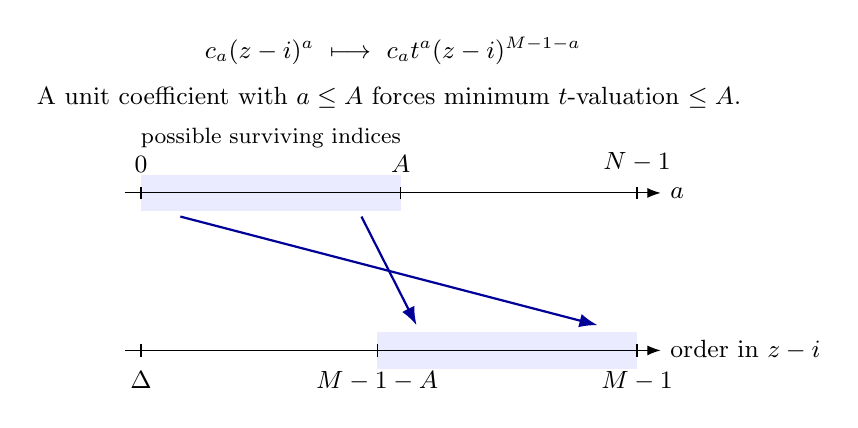
\begin{tikzpicture}[>=Latex,font=\small,x=1cm,y=1cm]
\fill[blue!8] (0,-.23) rectangle (3.3,.23);
\fill[blue!8] (3.0,-2.23) rectangle (6.3,-1.77);
\draw[->] (-.2,0)--(6.6,0) node[right] {$a$};
\draw[->] (-.2,-2)--(6.6,-2) node[right] {order in $z-i$};
\foreach \x/\lab in {0/0,3.3/A,6.3/{N-1}} {
 \draw (\x,-.08)--(\x,.08);
 \node[above=4pt] at (\x,0) {$\lab$};
}
\draw (0,-2.08)--(0,-1.92);
\node[below=4pt] at (0,-2) {$\Delta$};
\draw (3,-2.08)--(3,-1.92);
\node[below=4pt] at (3,-2) {$M-1-A$};
\draw (6.3,-2.08)--(6.3,-1.92);
\node[below=4pt] at (6.3,-2) {$M-1$};
\draw[->,blue!60!black,thick] (.5,-.3)--(5.8,-1.68);
\draw[->,blue!60!black,thick] (2.8,-.3)--(3.5,-1.68);
\node[anchor=south,font=\footnotesize] at (1.65,.45) {possible surviving indices};
\node[align=center,anchor=south] at (3.15,.95) {A unit coefficient with $a\leq A$ forces minimum $t$-valuation $\leq A$.};
\node[anchor=south] at (3.2,1.5) {$c_a(z-i)^a\ \longmapsto\ c_at^a(z-i)^{M-1-a}$};
\end{tikzpicture}
\caption{Taylor reversal in the expansion argument (schematic, not to scale). For a normalized input with integral Taylor coefficients and a unit among $a\leq A$, every term surviving in the leading reduction of its image has $a\leq A$. The reduction therefore vanishes to order at least $M-1-A$ at $i$. The proof applies this to every vector in a $j$-dimensional subspace, with $A=a_{ij}$.}
\label{fig:taylor-reversal}
\end{figure}


This conclusion controls the whole reduction $\overline{T_iU'}$.
Indeed, every nonzero $v\in T_iU'$ has a preimage $f\in U'$.  Normalizing
$f$ multiplies $v$ by the same power of $t$, so the leading reduction
of $v$ is exactly the leading reduction already considered.  An integral
$v$ reduces either to this leading reduction or to zero.  We have not
assumed that $T_i(U'\cap\mathcal O^N)$ is the full integral lattice of
$T_iU'$.  By injectivity of $T_i$ and
Lemma~\ref{lem:integral-reduction}, $\overline{T_iU'}$ has dimension $j$.
It lies in $\overline W$ and in its vanishing filtration of order at
least $M-1-A$.  Formula~\eqref{eq:vanishing-filtration} now gives
\eqref{eq:order-reversal}.

For each fixed $i$, summing \eqref{eq:order-reversal} over $j=1,\ldots,k$
uses the largest $k$ distinct orders of the same space $\overline W$.
The remaining orders are nonnegative.  Although the auxiliary spaces
$U'$ may depend on $j$, these are bounds on the fixed filtration of
$\overline W$ and can therefore be summed.  Applying
Lemma~\ref{lem:wronskian-orders} to both reduced spaces gives
\begin{align*}
  \ell(M-1)+w\binom\ell2
  &\geq\sum_{i=0}^n\sum_{h=1}^{\ell}b_{ih}\\
  &\geq wk(M-1)-\sum_{i=0}^n\sum_{j=1}^k a_{ij}\\
  &\geq wk(M-1)-k(N-1)-w\binom k2\\
  &=(w-1)k(M-1)+k\Delta-w\binom k2.
\end{align*}
If $\ell\leq(w-1)k$, this implies
\[
  k\Delta\leq w\left(\binom k2+\binom\ell2\right)
  \leq\frac w2\bigl(1+(w-1)^2\bigr)k^2
  \leq\frac{w^3}{2}Bk
  <2w^3Bk=k\Delta,
\]
a contradiction.  This proves the strict expansion bound.
\end{proof}

\subsection{From expansion to the rank bound}

The proof uses the standard shrunk-subspace obstruction: if every
coefficient matrix sends a common subspace into one of smaller
dimension, no matrix substitution can be invertible.
This is the elementary obstruction direction of the
noncommutative-rank characterization of Fortin and
Reutenauer~\citep[Section~2, Theorem~1]{FR04}; see also
\citet[Definition~1.1 and Section~5.1]{IQS18}.
We derive the obstruction from expansion and give the required
extension-field comparison explicitly.

\begin{proof}[Proof of Proposition~\ref{prop:rectangular}]
Suppose that $\sum_iA_i\otimes T_i$ has a nonzero kernel vector,
written as $q$ components $f_1,\ldots,f_q\in\mathcal P_N(F)$.  Let
$U$ be their span, of dimension $1\leq k\leq q\leq B$, and choose
a basis $u_1,\ldots,u_k$ of $U$.  Write
\[
  f_\alpha=\sum_{j=1}^k P_{\alpha j}u_j,
  \qquad P\in\Mat_{q\times k}(F).
\]
Since the $f_\alpha$ span $U$, the matrix $P$ has rank $k$.  Each
row of the concatenated matrix
\[
  C=[\,A_0P\ \ A_1P\ \ \cdots\ \ A_nP\,]
\]
is a relation among the $wk$ vectors $T_i u_j$: this is exactly the
corresponding component of the kernel equation.  Those vectors span
$\sum_iT_iU$, whose dimension is greater than $(w-1)k$ by
Lemma~\ref{lem:small-expansion}.  Their relation space therefore has
dimension less than $k$, and hence $\rank C<k$.

Let $V$ be the column space of $P$ and $V_-$ the column space of $C$,
both in $F^q$.  Equality of row rank and column rank yields
\begin{equation}
  \dim_F V=k,\qquad \dim_FV_-<k,
  \qquad A_iV\subseteq V_-\quad(0\leq i\leq n).
  \label{eq:shrunk-subspace}
\end{equation}
Thus every coefficient matrix sends the same input subspace into a
strictly smaller common output subspace.

To compare this obstruction with the given witness over $E$, introduce
a fresh formal variable $\tau$ and work in $J=E((\tau))$.  Embed $E$
as the constant series and embed $F$ by
\[
  \sum_m q_m t^m\longmapsto\sum_m q_m\tau^m.
\]
These embeddings agree on $\Q$, which contains all the $A_i$.  A
transcendental element already in $E$, even one named $t$, remains a
coefficient and is not identified with $\tau$.  The embeddings preserve
matrix ranks, since nonzero minors stay nonzero.  Denote the extended
subspaces in \eqref{eq:shrunk-subspace} by $V_J$ and $(V_-)_J$.
Putting $X_0=I_e$, the witness evaluation maps
\[
  \left(\sum_{i=0}^n A_i\otimes X_i\right)
       (V_J\otimes_J J^e)
  \subseteq (V_-)_J\otimes_J J^e.
\]
The domain on the left has dimension $ke$, and the space on the right
has dimension strictly less than $ke$.  This contradicts invertibility
of the witness matrix, whose inverse over $E$ remains an inverse over
$J$.  The rectangular evaluation is therefore injective.

In the padded evaluation $\sum_iA_i\otimes R_i(t)$, selecting the
first $N$ columns within each of the $q$ blocks recovers the rectangular
evaluation.  Its rank over $F$ is at least $qN$.  The corresponding
nonzero maximal minor belongs to $\Q[t]$, so it is also nonzero over
$\Q(t)$.  In particular, no coefficient of the formal subspaces or
their bases has to be specialized.  Finally,
\[
  qN-(q-1)M=M-q\Delta\geq M-B\Delta>0,
\]
which proves \eqref{eq:padded-rank}.
\end{proof}

\section{Deformation inside a division algebra}\label{sec:division}

The rank bound from Proposition~\ref{prop:rectangular} is close to full
rank.  We now deform the test matrices so that every possible rank is a
multiple of their block size.  The same deformation will also turn a
defined nonzero value of a rational formula into an invertible value over
an extension field.
The construction is a form of the generic cyclic, or symbol,
division algebra. Explicit split representations and block-rank
divisibility appear in the constructive regularity methods of
Ivanyos, Qiao, and Subrahmanyam~\citep[Sections~4.3 and~5.2 of the
preprint]{IQS17}; see also their later regularity
algorithm~\citep[Section~4]{IQS18}.
Division-algebra witnesses and invertible hits are also used in
rational-formula black-box testing by Arvind, Chatterjee, and
Mukhopadhyay~\citep{ACM22,ACM25}.
Here the needed deformation and rank-divisibility statement have
a direct proof using two explicit matrices. This matrix embedding
is distinct from the rational multiplication representation in
Section~\ref{sec:generator}.

\begin{lemma}[A matrix lift into a division algebra]\label{lem:division-lift}
Let $d\geq 1$, let $K$ be a field of characteristic zero, and let
$\omega\in K$ be a primitive $d$th root of unity.  On the standard basis
$e_0,\ldots,e_{d-1}$ of $K^d$, with subscripts taken modulo $d$, set
\[
  De_j=\omega^j e_j,
  \qquad Se_j=e_{j+1}.
\]
For algebraically independent indeterminates $p,r$ over $K$, there is a
division algebra
\[
  \mathcal D\subseteq\Mat_d\bigl(K(p,r)\bigr)
\]
containing, for every $R\in\Mat_d(K)$, the matrix
\begin{equation}\label{eq:division-lift}
  R^*=\sum_{a,b=0}^{d-1}c_{ab}p^a r^bD^aS^b,
  \qquad
  c_{ab}=\frac1d\sum_{j=0}^{d-1}\omega^{-aj}R_{j,j-b}.
\end{equation}
The matrix $R^*$ specializes to $R$ at $p=r=1$.
Moreover, $\mathcal D$ has dimension $d^2$ over the central subfield
$K(p^d,r^d)$, and every matrix with blocks in $\mathcal D$ has rank over
$K(p,r)$ divisible by $d$.
\end{lemma}

\begin{proof}
For each $b$, the only potentially nonzero entries of $D^aS^b$ have the
form
\[
  (D^aS^b)_{j,j-b}=\omega^{aj}.
\]
The identity
\[
  \sum_{j=0}^{d-1}\omega^{(a-a')j}
  =\begin{cases}d,&a=a',\\0,&a\ne a',\end{cases}
  \qquad 0\leq a,a'<d,
\]
therefore gives Fourier inversion separately on each of these cyclic
diagonals.  In particular, the $d^2$ matrices $D^aS^b$ form a basis of
$\Mat_d(K)$, with the coefficients displayed in
\eqref{eq:division-lift}.  This proves the asserted specialization.

Put $X=pD$ and $Y=rS$, and let $\mathcal A$ be the unital
$K$-algebra they generate inside $\Mat_d(K(p,r))$.  Since
$DS=\omega SD$, we have
\begin{equation}\label{eq:division-monomials}
  XY=\omega YX,
  \qquad
  (X^iY^j)(X^kY^\ell)
    =\omega^{-jk}X^{i+k}Y^{j+\ell}
  \quad(i,j,k,\ell\geq0).
\end{equation}
Thus the ordered monomials $X^iY^j$ span $\mathcal A$ over $K$.
They are also linearly independent: in any finite relation, the
coefficient of the scalar monomial $p^i r^j$ is the corresponding
scalar coefficient times the invertible constant matrix $D^iS^j$.
Algebraic independence of $p,r$ forces each such coefficient to vanish.

Order the exponent pairs lexicographically.  For two nonzero elements
of $\mathcal A$, the largest exponent in their product is the sum of
their largest exponents, by \eqref{eq:division-monomials}.  Its
coefficient is the product of two nonzero coefficients and a nonzero
power of $\omega$.  Hence $\mathcal A$ has no zero divisors.

The elements
\[
  X^d=p^dI_d,
  \qquad Y^d=r^dI_d
\]
are scalar matrices.  We may consequently invert every nonzero
element of the central polynomial ring $K[p^d,r^d]I_d$ and obtain a
subalgebra $\mathcal D$ of $\Mat_d(K(p,r))$.  Every element of this
localization can be written $a/z$ with $a\in\mathcal A$ and
$0\ne z\in K[p^d,r^d]$.  Products of nonzero such fractions remain
nonzero, so $\mathcal D$ still has no zero divisors.

Let $F_0=K(p^d,r^d)$.  Reducing the exponents of $X,Y$ modulo $d$
shows that
\begin{equation}\label{eq:division-central-basis}
  \{X^aY^b:0\leq a,b<d\}
\end{equation}
spans $\mathcal D$ over $F_0$.  To see independence over $F_0$,
clear a common denominator in a proposed relation.  Expanding the
resulting coefficients in $K[p^d,r^d]$ gives a relation among the
ordered monomials over $K$; distinct pairs $(a,b)$ in
\eqref{eq:division-central-basis} have distinct exponent residues
modulo $d$.  All its coefficients must therefore vanish.
It follows that $\dim_{F_0}\mathcal D=d^2$.

For a nonzero $z\in\mathcal D$, left and right multiplication by $z$
are injective $F_0$-linear maps from this finite-dimensional space to
itself, and hence are surjective.  There exist $b,c\in\mathcal D$
with $zb=1$ and $cz=1$, and associativity gives
$c=c(zb)=(cz)b=b$.  Thus $z$ has a two-sided inverse in
$\mathcal D$.  This proves that $\mathcal D$ is a division algebra.
Since $p^ar^bD^aS^b=X^aY^b$, every lift in
\eqref{eq:division-lift} belongs already to $\mathcal A$.

Finally, consider an arbitrary block matrix with entries in
$\mathcal D$.  If it has a nonzero block, move that block to the
first position by block row and column permutations.  Writing the
result as
\[
  \begin{pmatrix}a&b\\c&E\end{pmatrix},\qquad a\ne0,
\]
block elimination gives
\[
  \begin{pmatrix}1&0\\-c&I\end{pmatrix}
  \begin{pmatrix}a^{-1}&0\\0&I\end{pmatrix}
  \begin{pmatrix}a&b\\c&E\end{pmatrix}
  \begin{pmatrix}1&-a^{-1}b\\0&I\end{pmatrix}
  =
  \begin{pmatrix}1&0\\0&E-ca^{-1}b\end{pmatrix}.
\]
All blocks and all these invertible operations remain in
$\mathcal D$.  Iterating reduces the matrix to identity blocks and
zero blocks.  Each identity block is an ordinary $d\times d$
identity matrix, and the operations are invertible over $K(p,r)$
as well.  Its ordinary rank is therefore $d$ times the number of
identity blocks, as required.
\end{proof}

The scalar fields in this lemma have different roles.  Finite
dimensionality and the division property are proved over the central
field $K(p^d,r^d)$.  Ordinary matrix rank is measured over the larger
field $K(p,r)$ in the given embedding.  The elimination proof uses
only operations in $\mathcal D$; it does not enlarge that algebra by
arbitrary scalars from $K(p,r)$.

\begin{proposition}[Full-rank deformed pencils]\label{prop:pencil-deformation}
Fix a primitive $M$th root of unity $\omega\in\C$, and lift the
padded matrices $R_0(t),\ldots,R_n(t)$ by
Lemma~\ref{lem:division-lift} with $d=M$ and
$K=\Q(\omega)(t)$.  Let
\[
  L(x)=A_0+\sum_{i=1}^n A_i x_i,
  \qquad A_i\in\Mat_q(\Q),\qquad 1\leq q\leq B,
\]
be an affine pencil admitting an invertible matrix evaluation over
some extension field of $\Q$.  Then
\begin{equation}\label{eq:deformed-pencil-determinant}
  P_{L,\omega}(t,p,r)
   :=\det\!\left(\sum_{i=0}^n A_i\otimes R_i^*(t,p,r)\right)
   \ne0.
\end{equation}
This is a polynomial in $\Q(\omega)[t,p,r]$ of total degree at most
$3BM^2$.  In particular $\det R_0^*$ is a nonzero polynomial.
\end{proposition}

\begin{proof}
Proposition~\ref{prop:rectangular} gives
\[
  \rank_{\Q(t)}\left(\sum_{i=0}^n A_i\otimes R_i(t)\right)
      \geq qN>(q-1)M.
\]
Choose a nonzero minor of order greater than $(q-1)M$.
It remains nonzero over $\Q(\omega)(t)$.  The corresponding minor
of the lifted matrix specializes to it at $p=r=1$, so the lifted
minor is not identically zero.  The lifted matrix consequently has
rank greater than $(q-1)M$ over $\Q(\omega)(t,p,r)$.

Its $M\times M$ blocks belong to the division algebra of
Lemma~\ref{lem:division-lift}: each is a rational linear combination
of the $R_i^*$.  Its rank is thus a multiple of $M$.  As the whole
matrix has order $qM$, its rank must be $qM$, proving
\eqref{eq:deformed-pencil-determinant}.

The entries of $R_i(t)$ lie in $\mathbb Z[t]$ and have degree at
most $N-1$.  The Fourier coefficients in
\eqref{eq:division-lift} introduce only the constant denominator
$M$, while the factors $p^ar^b$ have total degree at most $2(M-1)$.
Every lifted entry is therefore a polynomial of total degree at
most $N-1+2(M-1)<3M$.  A determinant of order $qM$ has total degree
at most $3qM^2\leq3BM^2$.

For the last assertion, apply the result to the order-one constant
pencil $L=1$, whose coefficient $A_0$ is $1$ and whose other
coefficients vanish.  Its determinant in
\eqref{eq:deformed-pencil-determinant} is exactly $\det R_0^*$.
\end{proof}

At any specialization at which $R_0^*$ is invertible, set
$X_i=(R_0^*)^{-1}R_i^*$ for $1\leq i\leq n$.  The identity
\begin{equation}\label{eq:division-left-normalization}
  A_0\otimes I_M+\sum_{i=1}^n A_i\otimes X_i
  =
  \bigl(I_q\otimes(R_0^*)^{-1}\bigr)
  \left(\sum_{i=0}^n A_i\otimes R_i^*\right)
\end{equation}
shows that simultaneous nonvanishing of the determinant constraints
in Proposition~\ref{prop:pencil-deformation}, including the
constant-pencil constraint, makes the corresponding affine pencils
invertible on this normalized tuple.  The order of multiplication
in \eqref{eq:division-left-normalization} is part of the identity.

\begin{lemma}[An invertible witness for a nonzero formula]
\label{lem:invertible-witness}
Every admissible nonzero rational formula over $\Q$ has a defined
evaluation at matrices over an extension field of $\Q$ for which
its value is invertible.
\end{lemma}

\begin{proof}
By the definition of nonzero, there is a tuple
$W=(W_1,\ldots,W_n)$ of rational matrices of some common dimension
$d\geq1$ at which the given formula is defined and has nonzero
value.  Choose a primitive $d$th root $\omega$, put $K=\Q(\omega)$,
and lift each $W_i$ to $W_i^*$ by
Lemma~\ref{lem:division-lift}.

We first verify the domain of the actual formula tree independently
of the division-algebra argument.  Inside $K(p,r)$ consider the
commutative ring
\[
  \mathcal O=
  \left\{\frac{f}{g}: f,g\in K[p,r],\ g(1,1)\ne0\right\}.
\]
Evaluation at $(1,1)$ is a ring homomorphism
$\varepsilon:\mathcal O\to K$.  An element of $\mathcal O$ whose
image under $\varepsilon$ is nonzero is a unit in $\mathcal O$:
if it is written $f/g$, then $f(1,1)\ne0$ and its inverse is $g/f$.

We claim, by induction up the original tree, that each subtree
evaluated at the lifted inputs gives a matrix over $\mathcal O$
whose image under $\varepsilon$ is its value at $W$.
This holds for leaves by the specialization property of the lift,
and is preserved by addition and ordered multiplication.  At an
inverse gate, let $G\in\Mat_d(\mathcal O)$ be the already
constructed value of the child.  Since the original evaluation is
defined, $\varepsilon(G)$ is invertible.  Consequently
\[
  \varepsilon(\det G)=\det\varepsilon(G)\ne0,
\]
so $\det G$ is a unit of $\mathcal O$.  The formula
\[
  G^{-1}=\frac{\operatorname{adj}(G)}{\det G}
\]
then constructs its inverse in $\Mat_d(\mathcal O)$ and gives the
correct specialized inverse.  This proves the claim at every
inverse gate, regardless of its nesting depth.

The lifted formula is therefore defined over $K(p,r)$.  Its final
matrix is nonzero, because one of its entries specializes to a
nonzero entry of the original final value.

Now use the division algebra $\mathcal D$ from
Lemma~\ref{lem:division-lift}.  Every lifted input and every
rational scalar constant belongs to $\mathcal D$.  A second
induction shows that every intermediate value belongs to
$\mathcal D$: sums and products stay in it, and an operand at an
inverse gate is already known to be invertible as an ambient
matrix, hence is nonzero in $\mathcal D$.  Its inverse in
$\mathcal D$ equals its ordinary matrix inverse by uniqueness.
The final nonzero value is thus a nonzero element of a division
algebra, and is invertible as a matrix over $K(p,r)$.
\end{proof}

Only those entries proved to lie in $\mathcal O$ are specialized in
this argument.  No specialization map on the whole division algebra
is needed.  In particular, the inverse of the final value may have
a pole at $(1,1)$ when the original nonzero value is singular; its
invertibility is asserted only at the lifted tuple over the
extension field.  If $d=1$, the lift leaves every input scalar
unchanged, and a nonzero scalar final value is already invertible.
The witness dimension $d$ in Lemma~\ref{lem:invertible-witness} is
purely existential and need not be bounded.  The matrices used in
the construction instead have the predetermined block size $M$.

\section{Encoding a formula and its evaluation domain}
\label{sec:encoding}

We now turn the conditions imposed by a rational formula into finitely many
affine-pencil invertibility conditions.  We keep the original formula tree:
an inverse gate must have an invertible operand even when its contribution
later cancels or is multiplied by zero.
Affine-matrix representations of free-field elements appear in
Cohn and Reutenauer~\citep[Section~3.1]{CR94}.
Linear realizations by block inverses and tests for the original domain
appear in Hrube\v{s} and Wigderson~\citep[Theorem~2.6, Section~6,
and Proposition~7.1]{HW15}. Their domain criterion retains pencils
for all gate subformulas. We give the recursions and the domain
argument in full for the precise tree-size convention used here,
and show why the inverse-node pencils together with one root
augmentation suffice. The argument concerns the given tree and
requires no domain-preserving balancing transformation.

For a subtree $h$, let $|h|$ denote its number of vertices, let $\lambda(h)$
denote its number of leaves, and let $\iota(h)$ denote its number of inverse
gates.  Each occurrence of a subtree is treated separately.  A pencil of
order $q$ has the form
\[
 L(x)=A_0+\sum_{i=1}^n A_i x_i,
 \qquad A_0,\ldots,A_n\in\Mat_q(\Q).
\]
At a tuple $X=(X_1,\ldots,X_n)$ of matrices of order $d$ over a field
extension of $\Q$, its evaluation is
\[
 L(X)=A_0\otimes I_d+\sum_{i=1}^n A_i\otimes X_i.
\]
When a constant row $u$ or column $v$ is used with such an evaluation, we
write $u$ and $v$ for $u\otimes I_d$ and $v\otimes I_d$, respectively.
Thus the expression $uL(X)^{-1}v$ is a matrix of order $d$.

\begin{lemma}[Affine realization of a subtree]
\label{lem:formula-realization}
For each subtree $h$ there are an affine pencil $L_h$ of order $q_h$, a
constant rational row $u_h$ of length $q_h$, and a constant rational column
$v_h$ of length $q_h$, such that
\begin{equation}
 q_h=2\lambda(h)+\iota(h)=|h|+1.
 \label{eq:realization-order}
\end{equation}
At every matrix tuple over every field extension of $\Q$ where the
original subtree $h$ is defined, $L_h$ is invertible and
\begin{equation}
 h=u_hL_h^{-1}v_h.
 \label{eq:realization-invariant}
\end{equation}
\end{lemma}

\begin{proof}
Here are the constructions, followed by verification of the invariant.
All zero blocks have the sizes prescribed by the adjacent blocks.

\emph{Leaf.}  If $h$ is a variable or a rational constant, set
\[
 L_h=\begin{pmatrix}1&-h\\0&1\end{pmatrix},
 \qquad u_h=\begin{pmatrix}1&0\end{pmatrix},
 \qquad v_h=\begin{pmatrix}0\\1\end{pmatrix}.
\]

\emph{Addition.}  For $h=f+g$, set
\[
 L_h=\begin{pmatrix}L_f&0\\0&L_g\end{pmatrix},
 \qquad u_h=\begin{pmatrix}u_f&u_g\end{pmatrix},
 \qquad v_h=\begin{pmatrix}v_f\\v_g\end{pmatrix}.
\]

\emph{Ordered multiplication.}  For $h=fg$, set
\[
 L_h=\begin{pmatrix}L_f&-v_fu_g\\0&L_g\end{pmatrix},
 \qquad u_h=\begin{pmatrix}u_f&0\end{pmatrix},
 \qquad v_h=\begin{pmatrix}0\\v_g\end{pmatrix}.
\]

\emph{Inversion.}  For $h=g^{-1}$, set
\[
 L_h=\begin{pmatrix}L_g&v_g\\u_g&0\end{pmatrix},
 \qquad u_h=\begin{pmatrix}0&-1\end{pmatrix},
 \qquad v_h=\begin{pmatrix}0\\1\end{pmatrix},
\]
where the zero part of each selector has length $q_g$.  Equivalently,
$u_h=-e_{q_g+1}^{\mathsf T}$ and $v_h=e_{q_g+1}$.

The rows and columns just specified are constant.  In particular,
$v_fu_g$ is a constant matrix, so every displayed pencil is affine in
the original variables.  No multiplication of variable entries is
introduced into a pencil.

Fix an evaluation tuple and prove the invariant by induction on the
subtree.  A leaf pencil has inverse
$\left(\begin{smallmatrix}I_d&h\\0&I_d\end{smallmatrix}\right)$, and its selectors
give $h$.  At an addition gate, definedness of the gate implies
definedness of both children.  Their pencils are invertible by induction,
and block-diagonal inversion gives the sum of the two represented values.
At a multiplication gate, the same induction gives
\[
 L_h^{-1}=
 \begin{pmatrix}
  L_f^{-1}&L_f^{-1}v_fu_gL_g^{-1}\\
  0&L_g^{-1}
 \end{pmatrix}.
\]
The selected block is consequently
\[
 u_fL_f^{-1}v_fu_gL_g^{-1}v_g
   =(u_fL_f^{-1}v_f)(u_gL_g^{-1}v_g)=fg,
\]
with the required order of multiplication.

At an inverse gate $h=g^{-1}$, definedness means that $g$ is defined and
its value is invertible.  By induction $L_g$ is invertible and
$u_gL_g^{-1}v_g=g$.  The block factorization
\begin{equation}
 \begin{pmatrix}L_g&v_g\\u_g&0\end{pmatrix}
 =
 \begin{pmatrix}I&0\\u_gL_g^{-1}&I\end{pmatrix}
 \begin{pmatrix}L_g&0\\0&-g\end{pmatrix}
 \begin{pmatrix}I&L_g^{-1}v_g\\0&I\end{pmatrix}
 \label{eq:inverse-schur-factorization}
\end{equation}
shows that $L_h$ is invertible.  The lower-right block of its inverse is
$(-g)^{-1}=-g^{-1}$, so the negative row selector gives precisely
$g^{-1}$.  This proves the invariant in all four cases.

The orders are $2$ at leaves, add at binary gates, and increase by one
at inverse gates.  Hence $q_h=2\lambda(h)+\iota(h)$.  A rooted tree whose
internal vertices have one or two children has $\lambda(h)-1$ binary
vertices: counting edges both by vertices and by children gives this
identity.  Thus
\[
 |h|=\lambda(h)+(\lambda(h)-1)+\iota(h)
     =2\lambda(h)+\iota(h)-1,
\]
which proves~\eqref{eq:realization-order}.
\end{proof}

For the root formula $\Phi$, define its \emph{root augmentation} by
\begin{equation}
 J_\Phi=
 \begin{pmatrix}L_\Phi&v_\Phi\\u_\Phi&0\end{pmatrix}.
 \label{eq:root-augmentation}
\end{equation}
This has the same block form as an inverse-node pencil, but no inverse
gate is being added to the formula or counted in its size.

\begin{proposition}[Pencil certificates for the original formula tree]
\label{prop:formula-certificates}
Let $\Phi$ be a formula of size at most $s$, and put $B=2s+1$.  Form the
indexed collection $\mathcal C_\Phi$ consisting of $L_h$ for every
inverse-node occurrence $h$ of $\Phi$, together with $J_\Phi$.
Then:
\begin{enumerate}
 \item The collection contains at most $s+1$ affine pencils over $\Q$,
       each of positive order at most $B$.
 \item At every tuple of matrices of a common positive order over a
       field extension of $\Q$, all pencils in $\mathcal C_\Phi$ are
       invertible if and only if the original formula tree $\Phi$ is
       defined there and its value is invertible.
 \item If $\Phi$ is admissible and nonzero, there is a single tuple over
       some field extension of $\Q$ at which every pencil in
       $\mathcal C_\Phi$ is invertible.
\end{enumerate}
Adding the order-one constant pencil $1$ for normalization gives at
most $s+2$ pencils, still of order at most $B$, with the same simultaneous
feasibility property in the third assertion.
\end{proposition}

\begin{proof}
There are at most $s$ inverse-node occurrences.  By
Lemma~\ref{lem:formula-realization}, each corresponding pencil has order
$|h|+1\le s+1\le B$.  The augmentation has order
$|\Phi|+2\le s+2\le2s+1=B$, where the last inequality uses $s\ge1$.
This proves the first assertion.  The extra constant pencil has order
one and evaluates to an identity matrix at every tuple.

For one implication in the second assertion, assume that
$\Phi$ is defined and its value is invertible.  Each subtree is then
defined, so Lemma~\ref{lem:formula-realization} makes every inverse-node
pencil invertible.  The same lemma makes $L_\Phi$ invertible and gives
$u_\Phi L_\Phi^{-1}v_\Phi=\Phi$.  Applying
factorization~\eqref{eq:inverse-schur-factorization} at the root shows
that $J_\Phi$ is invertible, because its Schur complement is $-\Phi$.

Conversely, suppose all pencils in $\mathcal C_\Phi$ are invertible.
First establish that the original tree is defined, proceeding from
the leaves toward the root.  Leaves are always defined.  At an addition
or multiplication gate, both children have already been shown defined,
so the gate is defined.  At an inverse gate $h=g^{-1}$, all gates in
the child subtree have already been handled; in particular $g$ is
defined.  Lemma~\ref{lem:formula-realization} therefore makes $L_g$
invertible and represents $g$ by $u_gL_g^{-1}v_g$.  The pencil $L_h$ is
one of the assumed invertible pencils.  The two outer factors in
\eqref{eq:inverse-schur-factorization} are invertible, so the middle
factor is invertible as well.  It follows that $g$ is invertible, which
is exactly the condition needed for this inverse gate to be defined.

This induction proves definedness of the entire original tree.  It
also explains why no separate constraint on the pencil of an ordinary
subtree is needed: whenever that pencil is used, its invertibility
already follows from the established definedness of its subtree.
Now $L_\Phi$ is invertible by the realization lemma.  The assumed
invertibility of $J_\Phi$, whose Schur complement is $-\Phi$, forces
the final value $\Phi$ to be invertible.  This proves the reverse
implication without simplifying the formula or enlarging its domain.

Finally, if $\Phi$ is admissible and nonzero,
Lemma~\ref{lem:invertible-witness} supplies an evaluation over a field
extension of $\Q$ at which the original tree is defined and its value
is invertible.  The second assertion makes every pencil in
$\mathcal C_\Phi$ invertible at this one evaluation.  The constant
pencil $1$ is invertible there as well.  This proves the third assertion
and the normalization statement.
\end{proof}

\begin{remark}[Why every inverse occurrence is retained]
Consider the scalar expression
\[
 a=x^{-1},\qquad b=a^{-1},\qquad \Phi=b+1.
\]
It is undefined at $x=0$, although its simplified rational function is
$x+1$.  For the pencils above, direct computation gives
\[
 \det L_a=-x,\qquad \det L_b=1,\qquad \det J_\Phi=-(x+1).
\]
Thus the outer inverse pencil and the root augmentation alone would
accept $x=0$.  The retained inner inverse pencil $L_a$ rejects it.
Likewise, the formula $1+0\cdot x^{-1}$ retains the requirement that
$x$ be invertible.  The certificate collection is indexed by gates of
the given tree, including gates in branches whose later contributions
cancel.
\end{remark}

The witnesses and pencils in this section are used to prove the hitting
property; the generator will receive only $n,s$ and will not construct
them from an unknown formula.  The order and count bounds depend only
on the number of vertices.  They impose no restriction on inverse
nesting or on the bit lengths of the rational leaf constants.

\section{A rational hitting list and its bit complexity}
\label{sec:generator}

Proposition~\ref{prop:pencil-deformation} supplies polynomial matrices
$R_i^*(t,p,r)$ for which $\sum_i A_i\otimes R_i^*$ is invertible
over $\Q(\omega)(t,p,r)$ whenever the pencil
$A_0+\sum_{i=1}^n A_i x_i$ is feasible and has order at most~$B$.
We now replace the root-of-unity coefficients and specialize the
three parameters to obtain a single list of rational matrix tuples.
The parameters $w,B,\Delta,M,N$ retain their earlier definitions.

To remove the root of unity, we represent multiplication in a
finite-dimensional rational algebra. Over $\C$ this representation
is a direct sum of root evaluations, so our invertibility conditions
must hold simultaneously at all roots. Set
\begin{equation}
  \ell=\frac M2,\qquad D=M\ell=\frac{M^2}{2},\qquad
  H=1+3(s+2)BM^3,
  \qquad
  \mathcal R=\Q[\xi]/(\xi^\ell+1).
  \label{eq:generator-parameters}
\end{equation}
Here and below $\xi$ also denotes its residue class. In particular,
$\xi^\ell=-1$ and $\xi^M=1$, so every integral power of~$\xi$, including
a negative power, reduces to a signed member of the basis
$1,\xi,\ldots,\xi^{\ell-1}$.

\subsection{The rational representation and the generator}

Let $\Omega$ be the set of complex roots of $X^\ell+1$. Since $M$ is a
power of two, these are the $\ell$ distinct numbers
\[
  \exp\!\left(\frac{2\pi\mathrm{i}(2j+1)}{M}\right),
  \qquad 0\le j<\ell.
\]
Every one is a primitive $M$th root of unity: its exponent $2j+1$ is
coprime to~$M$. Evaluation at these roots is an algebra isomorphism
\begin{equation}
  \mathcal R\otimes_{\Q}\C
    \longrightarrow \prod_{\omega\in\Omega}\C,
  \qquad f\longmapsto \bigl(f(\omega)\bigr)_{\omega\in\Omega}.
  \label{eq:cyclotomic-splitting}
\end{equation}
Indeed, a polynomial of degree less than $\ell$ is uniquely determined
by its values at $\ell$ distinct points, and interpolation gives a
polynomial with any prescribed values there.

For $a\in\mathcal R$, let $\rho(a)\in\Mat_\ell(\Q)$ be the matrix of
multiplication by~$a$ in the power basis. This is a unital algebra
homomorphism. It is computed using only rational arithmetic and the
relation $\xi^\ell=-1$. To make its splitting explicit, let $V$ be the
evaluation matrix whose $(\omega,j)$ entry is $\omega^j$, for
$\omega\in\Omega$ and $0\le j<\ell$. Interpolation says that $V$ is
invertible, and
\begin{equation}
  V\rho(a)V^{-1}
    =\operatorname{diag}\bigl(a(\omega):\omega\in\Omega\bigr).
  \label{eq:regular-representation-splitting}
\end{equation}
If $Q\in\Mat_d(\mathcal R)$, write $\rho_d(Q)$ for the rational
$d\ell$ by $d\ell$ matrix obtained by applying $\rho$ to every entry.
First changing basis by $I_d\otimes V$, and then reordering the basis
to group together coordinates belonging to the same root, gives
\begin{equation}
  \rho_d(Q)\sim_{\C}
    \bigoplus_{\omega\in\Omega}Q(\omega).
  \label{eq:matrix-regular-splitting}
\end{equation}
In particular, $\rho_d(Q)$ is invertible if and only if every
$Q(\omega)$ is invertible. These complex basis changes are used to
prove this assertion; the generator will not compute them.

We use the lift of Lemma~\ref{lem:division-lift}, now with $\xi$ in
place of a primitive root. For clarity, it can be computed directly
over~$\mathcal R$. Number the coordinates from $0$ to $M-1$ and set
\[
  D_\xi e_j=\xi^j e_j,\qquad Se_j=e_{j+1},
\]
with indices taken modulo~$M$. For $0\le i\le n$ define
\begin{align}
  \widetilde c_{i,a,b}(t)
    &=\frac1M\sum_{j=0}^{M-1}
          \xi^{-aj}(R_i(t))_{j,j-b},
       &&0\le a,b<M,\notag\\
  \widetilde R_i(t,p,r)
    &=\sum_{a,b=0}^{M-1}
          \widetilde c_{i,a,b}(t)p^a r^bD_\xi^aS^b
       \in\Mat_M\bigl(\mathcal R[t,p,r]\bigr).
  \label{eq:universal-cyclotomic-lift}
\end{align}
Evaluating its coefficients at $\xi=\omega$ gives exactly the lifted
matrix $R_i^{*,\omega}(t,p,r)$ from
Proposition~\ref{prop:pencil-deformation}. In particular, no choice of
a complex root is needed to compute~\eqref{eq:universal-cyclotomic-lift}.

The generator, on input $1^n,1^s$, performs the following finite
computation in a fixed order.
\begin{enumerate}
  \item Compute the integer parameters and the explicit matrices
    $R_0(t),\ldots,R_n(t)$ of
    Proposition~\ref{prop:rectangular}.
  \item For each $(t_0,p_0,r_0)\in\{1,\ldots,H\}^3$, compute
    \[
      Z_i=\rho_M\bigl(\widetilde R_i(t_0,p_0,r_0)\bigr)
      \in\Mat_D(\Q),\qquad 0\le i\le n.
    \]
  \item If $Z_0$ is singular, emit nothing for this triple. Otherwise
    emit the tuple
    \begin{equation}
      \bigl(Z_0^{-1}Z_1,\ldots,Z_0^{-1}Z_n\bigr).
      \label{eq:generator-output}
    \end{equation}
\end{enumerate}
Denote the resulting list by $\mathcal H_{n,s}$. Repetitions are
harmless. Every tuple has the same positive matrix dimension~$D$.

\subsection{The hitting property}

\begin{proposition}
\label{prop:generator-hitting}
Every nonzero admissible formula of size at most~$s$ has a defined,
invertible evaluation at a tuple in~$\mathcal H_{n,s}$.
\end{proposition}

\begin{proof}
Fix one such formula~$\Phi$. By
Proposition~\ref{prop:formula-certificates}, there is a family of at
most $s+1$ affine linear pencils over~$\Q$, each of order at most~$B$,
whose simultaneous invertibility ensures that the original formula
tree is defined and has an invertible value. These are the pencils
of all inverse-node occurrences and the root augmentation. Each has
an invertible evaluation over an extension field. Add the order-one
constant pencil~$1$ to this family, and call the resulting family
$\widehat{\mathcal C}_\Phi$. Thus
$|\widehat{\mathcal C}_\Phi|\le s+2$.

For $L=A_0+\sum_{i=1}^n A_i x_i\in\widehat{\mathcal C}_\Phi$ and
$\omega\in\Omega$, recall from Proposition~\ref{prop:pencil-deformation} that
\[
  P_{L,\omega}(t,p,r)
    =\det\!\left(\sum_{i=0}^n
          A_i\otimes R_i^{*,\omega}(t,p,r)\right).
\]
Proposition~\ref{prop:pencil-deformation} says that each of these is
a nonzero polynomial of total degree at most~$3BM^2$. Regard all of
them as polynomials in the one integral domain $\C[t,p,r]$ and form
\[
  P_\Phi(t,p,r)
    =\prod_{L\in\widehat{\mathcal C}_\Phi}
       \prod_{\omega\in\Omega} P_{L,\omega}(t,p,r).
\]
This is a finite product of nonzero polynomials, and
\begin{equation}
  \deg P_\Phi
    \le (s+2)\frac M2\,3BM^2
    =\frac32(s+2)BM^3
    <H.
  \label{eq:generator-product-degree}
\end{equation}
The extension field used to witness invertibility of a pencil is
not part of this coefficient ring: the $A_i$ are rational, and the
displayed lift has coefficients in $\Q(\omega)$. Thus there is no
need to embed that witness field into~$\C$.

A nonzero polynomial in three variables of total degree less
than~$H$ cannot vanish on all of $\{1,\ldots,H\}^3$. To see this,
suppose it did. Fixing the last two coordinates gives a univariate
polynomial of degree less than~$H$ with $H$ roots, so every
coefficient in the first variable vanishes on the two-dimensional
grid. Repeating the same argument for the second and then the third
variable makes every coefficient zero, a contradiction.
Choose a triple at which $P_\Phi$ is nonzero.

At this triple every root evaluation of $\widetilde R_0$ is
invertible, by the factor corresponding to the constant pencil~$1$.
Equation~\eqref{eq:matrix-regular-splitting} therefore shows that
$Z_0$ is invertible, so the generator retains the triple. The same
equation, applied to each raw pencil, shows that
\[
  \sum_{i=0}^n A_i\otimes Z_i
\]
is invertible for every $L\in\widehat{\mathcal C}_\Phi$.
If $L$ has order~$q$, left multiplication gives the exact identity
\begin{equation}
  (I_q\otimes Z_0^{-1})
       \left(\sum_{i=0}^n A_i\otimes Z_i\right)
   =A_0\otimes I_D+
       \sum_{i=1}^n A_i\otimes(Z_0^{-1}Z_i).
  \label{eq:generator-normalization}
\end{equation}
Hence all the certificate pencils are invertible on the rational
tuple~\eqref{eq:generator-output}.

The preceding splitting proved invertibility after extending
scalars to~$\C$. For a rational matrix this implies that its rational
determinant is nonzero; the adjugate formula then supplies its
inverse over~$\Q$. We may consequently apply
Proposition~\ref{prop:formula-certificates} directly over~$\Q$ to the
output tuple. It makes every required inverse of the original tree
defined over~$\Q$ and makes the final value invertible. This also
shows why no assertion about preservation of arbitrary inverse
domains under a homomorphism is needed.
\end{proof}

\begin{corollary}
\label{cor:pencil-hitting}
Let $L=A_0+\sum_{i=1}^n A_i x_i$ be a rational affine linear pencil
of order $q\le B$ that admits an invertible matrix evaluation over
an extension field of~$\Q$. There is a tuple
$X\in\mathcal H_{n,s}$ for which $L(X)$ is invertible.
\end{corollary}

\begin{proof}
Use the same argument with the two pencils $L$ and~$1$.
The product of their determinant polynomials over all
$\omega\in\Omega$ is nonzero and has total degree at most
$3BM^3<H$. A grid point where this product is nonzero is retained
by the generator, and~\eqref{eq:generator-normalization} makes
$L$ invertible at its output tuple.
\end{proof}

The proof of Proposition~\ref{prop:generator-hitting} fixes $\Phi$
only after the list has been specified. Its
polynomial $P_\Phi$ is used solely to prove the existence of a good
triple in the fixed grid; the generator never constructs this
polynomial, the certificates, or a witness evaluation. Different
formulas may use different triples. Arbitrarily large rational
constants change the coefficients of $P_\Phi$, but neither its
degree bound nor the construction of~$\mathcal H_{n,s}$.

\Needspace{10\baselineskip}
\subsection{Bit complexity and output length}

\begin{proposition}
\label{prop:generator-complexity}
The list $\mathcal H_{n,s}$ can be constructed and written by one
deterministic Turing machine in a number of bit operations bounded
by a fixed polynomial in $n+s+1$. Its entire binary encoding has
length bounded by a fixed polynomial in the same quantity.
\end{proposition}

\begin{proof}
Put $m=n+s+1$. The parameter definitions give
\[
  w\le m,\qquad B\le2m,\qquad
  \Delta\le4m^4,\qquad M\le2B\Delta\le16m^5.
\]
Consequently
\begin{equation}
  H=O(m^{17}),\qquad D=O(m^{10}),\qquad
  H^3=O(m^{51}).
  \label{eq:generator-dimension-bounds}
\end{equation}
Counting the unary inputs, forming these parameters, and finding
$M$ by successive doubling all take polynomial time.

We first bound the integers actually computed at a grid triple.
For an input monomial $z^j$, where $0\le j<N$, the defining formula
for $T_i$ gives
\begin{equation}
  T_i z^j
    =\sum_{a=0}^j \binom ja i^{j-a}t^a(z-i)^{M-1-a}.
  \label{eq:generator-binomial-formula}
\end{equation}
Expanding each power in the monomial basis computes every entry
using integer arithmetic. Each coefficient in either of the two
basis expansions has absolute value at most $2^M w^M$. At a grid
value $1\le t\le H$, an entry of the padded matrix $R_i(t)$
therefore has absolute value at most
\[
  M\,2^{2M}w^{2M}H^M.
\]
In~\eqref{eq:universal-cyclotomic-lift}, the only division of a
coefficient is by~$M$. All powers of $\xi$ reduce to signed basis
monomials. The Fourier sum and the lift involve polynomially many
terms, and $p^a r^b\le H^{2M}$ on the grid. For example, the
absolute values of the power-basis coefficients of every entry of
$M\widetilde R_i(t,p,r)$ are bounded by
\[
  M^4\,2^{2M}w^{2M}H^{3M}.
\]
Multiplication by a power-basis monomial merely permutes those
coefficients and changes signs. Thus
\begin{equation}
  U_i:=MZ_i\in\Mat_D(\mathbb Z),\qquad
  b=O\!\left(M\log\bigl((w+1)(H+1)\bigr)+\log M\right)
    =O(m^5\log m)
  \label{eq:generator-input-bit-bound}
\end{equation}
is a common bound on the bit lengths of their entries. These
calculations have explicit nested loops of polynomial length:
binomial coefficients may be formed by Pascal's recurrence,
integer powers by repeated multiplication, and all ring
coefficients by the signed reductions just described. Every
intermediate sum and product in these loops has polynomial bit
length. The matrices $U_i$ can therefore be constructed in
polynomial bit time.

The common clearing factor cancels in normalization:
\begin{equation}
  Z_0^{-1}Z_i=U_0^{-1}U_i.
  \label{eq:generator-common-denominator}
\end{equation}
If $U_0$ is nonsingular, Cramer's rule computes each column of this
matrix using $\det U_0$ and determinants of $U_0$ with one column
replaced by a column of~$U_i$. All these are integer matrices of
order~$D$ with the same entry bit bound~$b$. Every minor of any such
matrix has absolute value at most $D!2^{Db}$. Hence its bit length
is bounded by
\begin{equation}
  \Lambda=O\bigl(D(b+\log(D+1))\bigr)
     =O(m^{15}\log m).
  \label{eq:generator-minor-bit-bound}
\end{equation}
Each output entry is a ratio of two such determinants. It can be
written with a signed binary numerator and a positive binary
denominator using $O(\Lambda)$ bits, changing both signs if
necessary. Cancelling their gcd is optional for this encoding.

For completeness, exact Gaussian elimination computes the needed
determinants in polynomial bit time without permitting fractions
to grow unchecked. Let $A$ be any one of these integer matrices.
After $k$ successful pivots, let $I_k$ be the ordered list of the
selected original row indices, and let
\[
  B_k=A[I_k,\{1,\ldots,k\}].
\]
This submatrix is invertible. For an unselected row index $u$ and
a column $v>k$, the remaining Gaussian entry is
\begin{equation}
  A_{uv}-A[u,\{1,\ldots,k\}]\,
         B_k^{-1}A[I_k,v]
   =\frac{
       \det\begin{pmatrix}
         B_k&A[I_k,v]\\
         A[u,\{1,\ldots,k\}]&A_{uv}
       \end{pmatrix}}
       {\det B_k}.
  \label{eq:generator-pivot-minors}
\end{equation}
For $k=0$ the denominator is~$1$ and the entry is $A_{uv}$.
The determinant identity follows by subtracting the appropriate
linear combination of the first $k$ block rows from the last row.
It also shows inductively that ordinary Gaussian updates compute
the displayed entries.

If the next pivot column has a nonzero remaining entry, swap its
row into the pivot position and append that original row index to
$I_k$. These swaps involve only unselected rows, so they do not
change any previously selected submatrix. Writing the next pivot
as~$p_{k+1}$, equation~\eqref{eq:generator-pivot-minors} gives
\[
  p_{k+1}=\frac{\det B_{k+1}}{\det B_k},
  \qquad p_1\cdots p_k=\det B_k.
\]
If the entire next remaining column is zero, the Schur complement
is singular and $\det A=0$. Otherwise all $D$ pivots can be taken,
and their product, multiplied by the sign of the accumulated row
permutation, equals~$\det A$.

Both the stored Gaussian entries and the accumulated pivot
products, when reduced to fractions, therefore have
$O(\Lambda)$-bit numerators and denominators: they are ratios of
minors or minors themselves. Each individual update combines only
a constant number of these fractions, so its intermediate products
and sums also have $O(\Lambda)$ bits before reduction. Integer
addition, multiplication, and division on such operands have
polynomial bit cost by the elementary digit algorithms. Gcd
reduction does as well: in the Euclidean algorithm the nonzero
remainders decrease by a factor of at least two within every two
steps, so there are $O(\Lambda)$ polynomial-cost divisions.
There are $O(D^3)$ Gaussian arithmetic updates. Pivot searches,
row swaps, and sign bookkeeping also have polynomial cost.
This proves polynomial bit time for each determinant, including
singular matrices and all the column-replaced matrices used by
Cramer's rule.

At each grid triple, at most $nD^2+1$ determinants suffice for the
singularity test and all output entries. Equations
\eqref{eq:generator-dimension-bounds}--\eqref{eq:generator-minor-bit-bound}
therefore give a fixed polynomial bound on the total computation.
The complete list contains at most $H^3 nD^2$ rational entries, so
its encoding length is
\begin{equation}
  O(H^3 nD^2\Lambda)=O(m^{87}\log m).
  \label{eq:generator-output-bit-bound}
\end{equation}
Dimensions, signs, and fixed delimiters fit within the same bound.
A fixed delimited encoding allows the list to be written as its
entries are produced; if its length is placed first, one may instead
buffer the polynomial-length list or make a preliminary counting
pass.

Finally, these arithmetic and loop bounds give a Turing-machine
bound as well. All arrays have polynomially many entries of
polynomial bit length. They may be stored as indexed binary records
on work tapes; even scanning all records for each requested access
adds only a fixed polynomial factor. The loops, elementary digit
algorithms, and delimiters are fixed in advance. Thus one
deterministic Turing machine performs the construction and writes
the whole list within $C(n+s+1)^k$ bit operations for some fixed
positive integers $C,k$. None of its arithmetic uses the constants
or coefficients of an unknown formula.
\end{proof}

\begin{proof}[Completion of the proof of Theorem~\ref{thm:main}]
Use the generator just defined. Proposition~\ref{prop:generator-hitting}
gives the universal hitting property, with invertible and therefore
nonzero output values. Proposition~\ref{prop:generator-complexity}
gives both required polynomial bounds, after increasing the same
fixed constants $C,k$ if necessary. The generator is deterministic
and depends only on its two unary inputs.
\end{proof}

\section{A universal rank-detecting list}
\label{sec:rank}

The hitting list and its complexity bounds are now established.
We use the pencil-hitting consequence to recover the exact
noncommutative rank of a rectangular affine pencil from one list
that is independent of all coefficient values. The additional input
is the characterization of free-field rank by normalized
matrix-evaluation ranks, recalled in the proof.

\begin{corollary}
\label{cor:rank-detecting-list}
Let $a,b\geq1$ and $k\geq0$, and put $P=a+b+k+1$. From these
parameters in unary, a deterministic generator constructs a nonempty
finite list $\mathcal R_{a,b,k}$ of pairs
\[
 (e,X),\qquad e\geq1,\quad
 X=(X_1,\ldots,X_k)\in\Mat_e(\Q)^k,
\]
in a fixed polynomial in $P$ bit operations. Its number of entries,
total binary encoding length, and every matrix dimension $e$ are
bounded by fixed polynomials in $P$. The list depends only on $a,b,k$.

For every rectangular rational affine pencil
\[
 A(x)=A_0+\sum_{i=1}^k A_i x_i,\qquad A_i\in\Q^{a\times b},
\]
write $\operatorname{ncrk}A$ for its rank over the free skew field on
$x_1,\ldots,x_k$ over $\Q$, with ordinary rational rank when $k=0$.
Then the exact identity
\begin{equation}
 \operatorname{ncrk}A
 =\max_{(e,X)\in\mathcal R_{a,b,k}}
   \frac{\rank_{\Q}\!\left(A_0\otimes I_e+
             \sum_{i=1}^k A_i\otimes X_i\right)}{e}
 \label{eq:rank-detecting-list}
\end{equation}
holds for all choices and bit lengths of the coefficients.

Suppose that, at each requested pair $(e,X)$, an oracle returns
either the complete exact rational $ae$ by $be$ matrix in
\eqref{eq:rank-detecting-list}, in binary rational encoding, or its
exact ordinary rank. Querying the whole list nonadaptively and taking
the maximum of the exact quotients returns $\operatorname{ncrk}A$.
If $L$ is the total binary length of the responses, list generation,
query writing, and response processing use $\operatorname{poly}(P+L)$
bit operations, in addition to the sum of the oracle's costs.
The response lengths and oracle costs may depend on the coefficient
heights. If $a=0$ or $b=0$, the rank is zero and no queries are needed.
\end{corollary}

\begin{proof}
\emph{Affine evaluations and free-field rank.}
Put
$H(z)=\sum_{i=0}^k A_i z_i$, with a new variable $z_0$.
The coefficient-span invariance of Fortin and
Reutenauer~\citep[Section~2, Corollary~1, and Section~3, Lemma~1]{FR04}
includes the constant coefficient: the free-field rank of a
rectangular affine linear matrix depends only on the span of all its
coefficient matrices. The coefficient spans of $A$ and $H$ are both
$\Span_{\Q}\{A_0,\ldots,A_k\}$, so their free-field ranks agree.
This uses coefficient-span invariance, not a specialization $z_0=1$
in a free skew field.

For $e\geq1$, let $h_e$ be the maximum rank of
$\sum_{i=0}^k A_i\otimes Z_i$ over $Z_i\in\Mat_e(\Q)$, and let
$\alpha_e$ be the maximum rank of
$A_0\otimes I_e+\sum_{i=1}^k A_i\otimes X_i$ over rational $X_i$.
Zero-padding the $A_i$ to square matrices of order $\max(a,b)$
preserves both free-field rank and every ordinary blow-up rank.
The homogeneous blow-up characterization and its attainment over
$\Q$~\citep[arXiv version, Definition~1.2 and its discussion,
Theorem~1.5]{IQS18} therefore give
\[
 r:=\operatorname{ncrk}A=\max_{e\geq1}\frac{h_e}{e},
\]
with the maximum attained. The tensor order used in that reference
differs from $A_i\otimes Z_i$ only by row and column permutations.
Here padding is used to preserve ranks, not to test invertibility.

For each fixed $e$, taking $Z_0=I_e$ gives $\alpha_e\leq h_e$.
If $h_e>0$, some $h_e$ by $h_e$ minor is a nonzero polynomial $p$
in the entries of the $Z_i$. The polynomial $p\det Z_0$ is nonzero;
since $\Q$ is infinite, it is nonzero at a rational tuple. There
$Z_0$ is invertible and the rank is $h_e$. Right multiplication gives
\[
 \left(\sum_{i=0}^k A_i\otimes Z_i\right)
       (I_b\otimes Z_0^{-1})
 =A_0\otimes I_e+\sum_{i=1}^k A_i\otimes(Z_iZ_0^{-1}),
\]
without changing rank. The case $h_e=0$ is immediate, so
$\alpha_e=h_e$ for every $e$. Consequently
\begin{equation}
 r=\max_{e\geq1}\frac{\alpha_e}{e}
 \label{eq:affine-normalized-rank}
\end{equation}
is attained: every individual affine evaluation has rank at most
$re$, and some rational evaluation has rank exactly $re$. No bound
on the dimension or entry heights of this existence witness
will be used.

\emph{Square completions for rank thresholds.}
For $0\leq t\leq\min(a,b)$, form the square affine pencil
\[
 C_t=\begin{pmatrix}A&U_t\\ V_t&0\end{pmatrix},
 \qquad U_t:a\times(a-t),\quad V_t:(b-t)\times b.
\]
The entries of $U_t,V_t$ are independent variables, so their
dimension-$e$ evaluations may be arbitrary matrices of the displayed
block sizes multiplied by $e$. For a fixed rational tuple $X$,
there exist rational choices of these completion blocks making
$C_t(X,U_t,V_t)$ invertible if and only if
$\rank A(X)\geq te$. Necessity follows by splitting the
completed matrix into its $A(X)$ and two off-diagonal blocks:
\[
 (a+b-t)e=\rank C_t(X,U_t,V_t)
 \leq\rank A(X)+(a-t)e+(b-t)e.
\]
For sufficiency, choose a $te$-dimensional subspace
$K\subseteq\Q^{be}$ on which $A(X)$ is injective. Take $V_t$ to be
surjective with kernel $K$, and take $U_t$ to map isomorphically onto
a complement of $A(X)K$ in $\Q^{ae}$. A vector in the kernel of the
completed matrix then has its first component in $K$, and the direct
sum $A(X)K\oplus\operatorname{im}U_t$ makes both components zero.
This proves invertibility. It includes $t=0$ and all empty-block
cases; in particular $C_0$ can always be made invertible.

\emph{A coefficient-independent list.}
Reserve $a^2$ variables $u_{ij}$ and $b^2$ variables $v_{ij}$,
disjoint from the first $k$ variables. For $C_t$, use the first
$a-t$ columns of the $u$-pool for $U_t$ and the first $b-t$ rows of
the $v$-pool for $V_t$. The pools can be reused for different $t$.
Thus every $C_t$ is a pencil in the same
$N=k+a^2+b^2$ variables, with unused variables allowed, and has
order $a+b-t\leq a+b$. Set $s=a+b$, so this order is at most
$B=2s+1$. Both $N$ and $s$ are positive. Apply the single list
$\mathcal H_{N,s}$ from Corollary~\ref{cor:pencil-hitting}, and
project each output onto its first $k$ matrices, retaining its
dimension $e$ and any repetitions. This defines $\mathcal R_{a,b,k}$;
it is nonempty because $C_0$ is feasible.

For $t=r$, equation~\eqref{eq:affine-normalized-rank} and the
completion criterion make $C_r$ feasible. A hit for $C_r$ therefore
has projected rank at least $re$, while every projected evaluation
has rank at most $re$. This proves~\eqref{eq:rank-detecting-list}
exactly, without rounding; individual ranks need not be divisible by
$e$. The argument includes $r=0$. When $k=0$, the projected tuple is
empty but still carries $e$, and the identity also follows directly
from $\rank(A_0\otimes I_e)=e\rank A_0$.

Since $N+s+1$ is polynomial in $P$, Proposition~\ref{prop:generator-complexity}
and the dimension bound~\eqref{eq:generator-dimension-bounds} give
the stated generation, query-encoding, and dimension bounds. The
generator never constructs $C_t$, learns $r$, or reads the
coefficients: $C_r$ is used only in the existence proof. For complete
matrix responses, exact rational elimination is polynomial in the
encoded response lengths and dimensions. For ordinary-rank responses,
only exact comparison of the rank/dimension quotients is needed.
These observations give the stated cost accounting.
\end{proof}

The assertion concerns exact matrix values or ordinary ranks, not
singularity-bit access to the original pencil. It makes no claim for
arbitrary rational circuits, finite fields, or total oracle-computation
bit time independent of coefficient heights. If complete scalar value
queries at zero and the standard basis points are also available, then
$k+1$ such queries reveal all coefficients, after which known
coefficient-aware rank algorithms apply with those bit lengths
counted~\citep[arXiv version, Theorem~1.5]{IQS18}. The distinct
conclusion here is the universal nonadaptive coefficient-independent
list, which also works with ordinary-rank responses.


\bibliographystyle{plainnat}
\bibliography{references}
\end{document}
